\section{Derivatives}

\subsection{Partial Derivatives}
The concept of \textit{derivatives} in functions in one variable is used to determine the change in the output of the
function as the input variable changes.

The concept of \textit{partial derivatives} is a generalization of the same idea in higher dimensions. They caputure the
rate of change of a function's output with respect to ONLY one variable at a time, holding all others constant.

For a real-valued function $f(x, y)$, the partial derivatives are as follows:

\begin{equation}
    \frac{\del f(x, y)}{\del x} = f_x = \lim_{h \to 0} \frac{f(x+h, y) - f(x, y)}{h}
\end{equation}

\begin{equation}
    \frac{\del f(x, y)}{\del y} = f_y = \lim_{h \to 0} \frac{f(x, y+h) - f(x, y)}{h}
\end{equation}

\begin{example}
    \normalfont Find the partial derivatives of $z = x^2 + 3xy + y - 1$ at $(4, -5)$.
    \begin{align*}
        \frac{\del z}{\del x} \bigg|_{(4, -5)} = z_x \big|_{(4, -5)} &= (2x + 3y) \big|_{(4, -5)} = -7 \\
        \frac{\del z}{\del y} \bigg|_{(4, -5)} = z_y \big|_{(4, -5)} &= (3x + 1) \big|_{(4, -5)} = 13
    \end{align*}
\end{example}

\begin{example}
    \normalfont Find the partial derivatives of $z$ with respect to $x$, given $yz - \text{ln}(z) = x + y$.

    Differentiating implicitly, we get
    $$yz_x - \frac{1}{z}z_x = 1 \implies z_x = \frac{1}{y - \frac{1}{z}}$$
\end{example}

\begin{example}
    \normalfont The plane $x = 1$ intersects the paraboloid $z = x^2 + y^2$ in a parabola. Find its slope at $(1, 3, 5)$.

    \begin{figure}[htp]
        \centering
        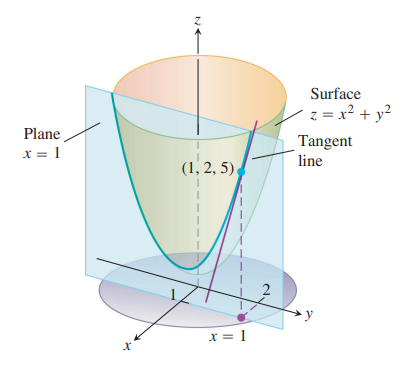
\includegraphics[scale=0.65]{example-6.1.3.png}
        \caption{The intersection of the plane $x=1$ and the paraboloid $z = x^2 + y^2$}
    \end{figure}

    The parabola formed at the intersection of $z = x^2 + y^2$ and $x = 1$ is $z = 1 + y^2$.
    The slope of the parabola so formed, at $(1, 3, 5)$ is:
    $$z_y \big|_{(1, 3, 5)} = 2y \big|_{(1, 3, 5)} = 6$$
\end{example}

\begin{example}
    \normalfont Given $f(x, y, z) = x \sin{(y + 3z)}$, find its partial derivative with respect to $z$.

    $$\frac{\del f(x, y, z)}{\del z} = f_z = 3x \cos{(y + 3z)}$$
\end{example}


\subsection{Higher-Order Partial Derivative}

\begin{enumerate}
     \item \textbf{Higher Partial Derivative} \\
    A $higher$ partial derivative is the partial derivative of a function with respect to the same variable multiple times.
    \begin{example}
        \normalfont $f_{xx},\ f_{yy},\ f_{xxx},\ f_{yyy},\ \hdots$
    \end{example}

    \item \textbf{Mixed Partial Derivative} \\
    A $mixed$ partial derivative is the partial derivative of a function with respect to different variables multiple times.
    \begin{example}
        \normalfont $f_{xy},\ f_{yx},\ f_{xxy},\ f_{xyx},\ f_{yyx},\ \hdots$
    \end{example}
\end{enumerate}

\begin{example}
    \normalfont Find the higher-order partial drivatives $f_{xy}$ and $f_{yx}$ for $f(x, y) = x\cos{y} + ye^x$.
    \begin{align*}
        f_x &= \cos{y} + ye^x &\ f_y &= -x\sin{y} + e^x \\
        f_{xy} &= -\sin{y} + e^x &\ f_{yx} &= -\sin{y} + e^x
    \end{align*}
\end{example}

\begin{theorem}
    [Mixed Derivative Theorem]
    If $f(x, y)$ and all its partial derivatives $f_x,\ f_y,\ f_{xy},$ and $f_{yx}$ are defined throughout an open region
    containing a point $\point \in \R^2$, and all are continuous at $\point$, then:
    \begin{equation}
        f_{xy}\point = f_{yx}\point.
    \end{equation}
\end{theorem}

\begin{example}
    \normalfont Find the second-order mixed partial derivative of $w(x, y) = xy + \frac{e^y}{y^2 + 1}$.
    \begin{align*}
        w_y &= x + \frac{1}{(y^2 + 1)^2} \left( \frac{e^y}{y^2 + 1} - \cdots \right) &\ w_x &= y + 0 \\
        w_{yx} &= 1 \text{ (as the term was a function of } y \text{)} &\ w_{xy} &= 1
    \end{align*}
\end{example}

\begin{theorem}
    [Increment Theorem for functions in two variables]
    In a region $R$ containing the point $\point$, the change in the value of the function $z = f(x, y)$ is given by
    \begin{equation}
        \Delta z = f(x_0 + \Delta x, y_0 + \Delta y) - f\point = (f_x \Delta x + f_y \Delta y) \big |_{\point}
    \end{equation}
\end{theorem}

\begin{theorem}
    [Chain Rule for more two variables]
    Provided that $w = f(x, y)$, and that $f_x$ and $f_y$ exist, then if $x = x(t)$ and $y = y(t)$, i.e. $x$ and $y$ are
    parametrized by $t$, then
    \begin{equation}
        \frac{dw}{dt} = f_x x_t + f_y y_t = \frac{\del f}{\del x} \frac{dx}{dt} + \frac{\del f}{\del y} \frac{dy}{dt}
    \end{equation}.
\end{theorem}

\begin{theorem}
    [Generalization of the Chain Rule]
    Provided that $w = f(x_1, x_2, \hdots, x_n)$, and that $f_{x_1}, f_{x_2}, \hdots, f_{x_n}$ exist, then if $x_i = x_i(t)$
    $\forall i \in \{1, 2, \hdots, n \}$, i.e. each $x_i$ is parametrized by $t$, then
    \begin{equation}
        \frac{dw}{dt} = \sum_{i=1}^n \frac{\del f}{\del x_i} \frac{dx_i}{dt}
    \end{equation}
\end{theorem}

\begin{example}
    \normalfont Find $w_t$ along $x = \sin{t}$ and $y = e^t$, given $w(x, y) = x^2y - y^2$.
    \begin{align*}
        w(t) &= e^t\sin^2{t} - e^{2t} &\ w(x, y) &= x^2y - y^2 \\
        w_t &= e^t\sin^2{t} + e^t\sin{2t} - 2e^{2t} &\ w_t &= 2xy(\cos{t}) + (x^2 - 2y)e^t \\
        &\ &\ w_t &= 2\sin{t}\cos{t} e^t + \sin^2{t} e^t - 2e^te^t \\
        &\ &\ w_t &= e^t\sin^2{t} + e^t\sin{2t} - 2e^{2t}
    \end{align*}
\end{example}


\subsection{Functions on a Surface}
A real-valued function in three variables is called a function on a \textit{surface}. Suppose the three variables, namely
$x, y, $ and $z$ are parametrized by $r$ and $s$. Then (say),

$$w = f(x, y, z);\text{ and } x = g(r, s),\ y = h(r, s), \text{ and } z = k(r, s)$$

Then,
\begin{align}
    \frac{dw}{dr} = \frac{\del f}{\del x} \frac{\del x}{\del r} + \frac{\del f}{\del y} \frac{\del y}{\del r} +
    \frac{\del f}{\del z} \frac{\del z}{\del r} = f_x x_r + f_y y_r + f_z z_r \\
    \frac{dw}{ds} = \frac{\del f}{\del x} \frac{\del x}{\del s} + \frac{\del f}{\del y} \frac{\del y}{\del s} +
    \frac{\del f}{\del z} \frac{\del z}{\del s} = f_x x_s + f_y y_s + f_z z_s
\end{align}

\begin{example}
    \normalfont Find $\frac{dw}{dr}$ if $w = x + 2y + z$, where $x = \frac{r}{s},\ y = r^2 + \text{ln}s$ and $z = 2r$.

    $$\frac{dw}{dr} = 1 \cdot \frac{1}{s} + 2 \cdot 2r + 1 \cdot 2 = \frac{1}{s} + 4r + 2$$
\end{example}

The same idea can be easily generalized to higher dimensions. Say, $w$ is a function of $n$-variables. Then,
$$w = f(x_1, x_2, \hdots, x_n); \text{ and } x_i = x_i(p_1, p_2, \hdots, p_m)$$

Then,
\begin{equation}
    \frac{dw}{dp_j} = \sum_{i = 1}^n f_{x_i} x_{i_{p_j}}, \text{ for some } 1 \leq j \leq m.
\end{equation}


\subsection{Implicit Differentiation}
Functions can be differentiated implictly to extract the rate of change of one variable with respect to another. However,
it is a tedious process.

\begin{theorem}
    [Formula for implicit differentiation]
    Suppose $F(x, y)$ is differentiable and that the equation $F(x, y) = 0$ defines $y$ as a differentiable function of $x$.
    Then, at any point where $f_y \neq 0$,
    \begin{equation}
        \frac{dy}{dx} = -\frac{F_x}{F_y}
    \end{equation}
\end{theorem}

\begin{example}
    \normalfont Find the derivative of $y$ with respect to $x$ given that $f(x, y) = y^2 - x^2 - \sin{(xy)} = 0$.
    $$\frac{dy}{dx} = -\frac{f_x}{f_y} = - \left( \frac{-2x - y\cos{(xy)}}{2y - x\cos{(xy)}} \right)
    = \frac{2x + y\cos{(xy)}}{2y - x\cos{(xy)}}$$
\end{example}